\section{Results} \label{sec:conclusions}
We produce simulated events until we find at least $100$ with sufficiently small localizations that further analysis is practical.
This cutoff is arbitrary, for all results reported we used a maximum volume of $0.5\times 10^{9}$\si{Mpc^3}.
We also observed values which had anomalously small localization volumes so we also constrained all simulated events to have a localization volume larger than $0.5\times 10^{7}$\si{Mpc^3}.
We found that a total of $650$ observations were needed to produce the desired $100$ well localized events.
These localized regions corresponded to $15.43\%$ of all generated samples.
In all of our tests we injected a known value of $H_0=70$\si{km.s^{-1}.Mpc^{-1}}.

\begin{figure}
    \centering
    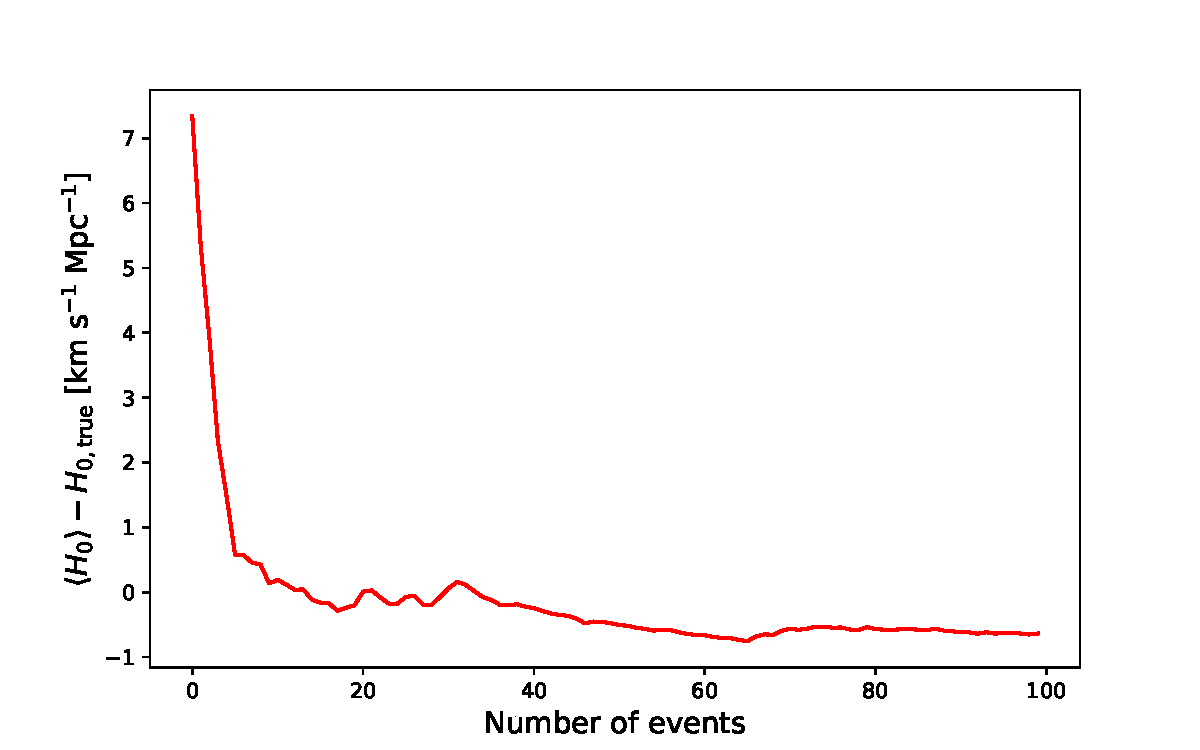
\includegraphics[width=0.9\columnwidth]{figures/diff.pdf}
    \caption{The deviation between the injected known value of $H_0$ and our expectation value based on $p(H_0 | d_{GW}, d_C)$.}
    \label{fig:mean_diff}
\end{figure}

\begin{figure}
    \centering
    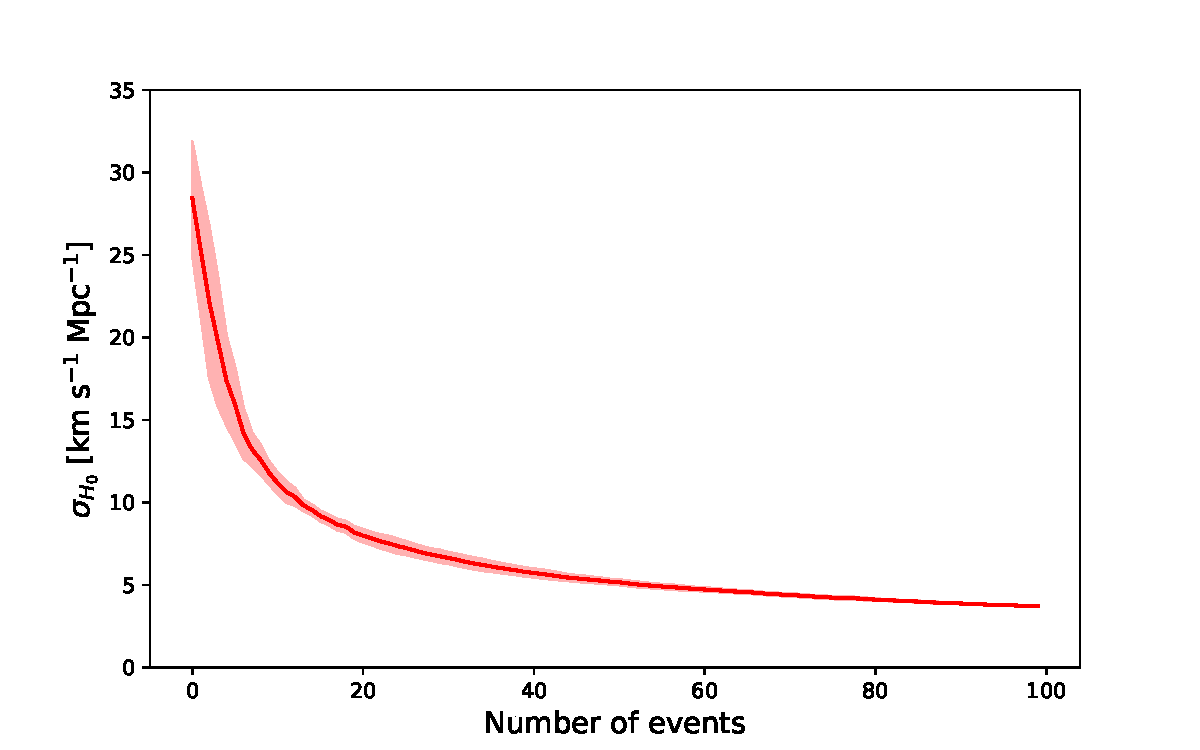
\includegraphics[width=0.9\columnwidth]{figures/std.pdf}
    \caption{The standard deviation obtained from the posterior $p(H_0 | d_{GW}, d_C)$.}
    \label{fig:std}
\end{figure}

\begin{figure*}
    \centering
    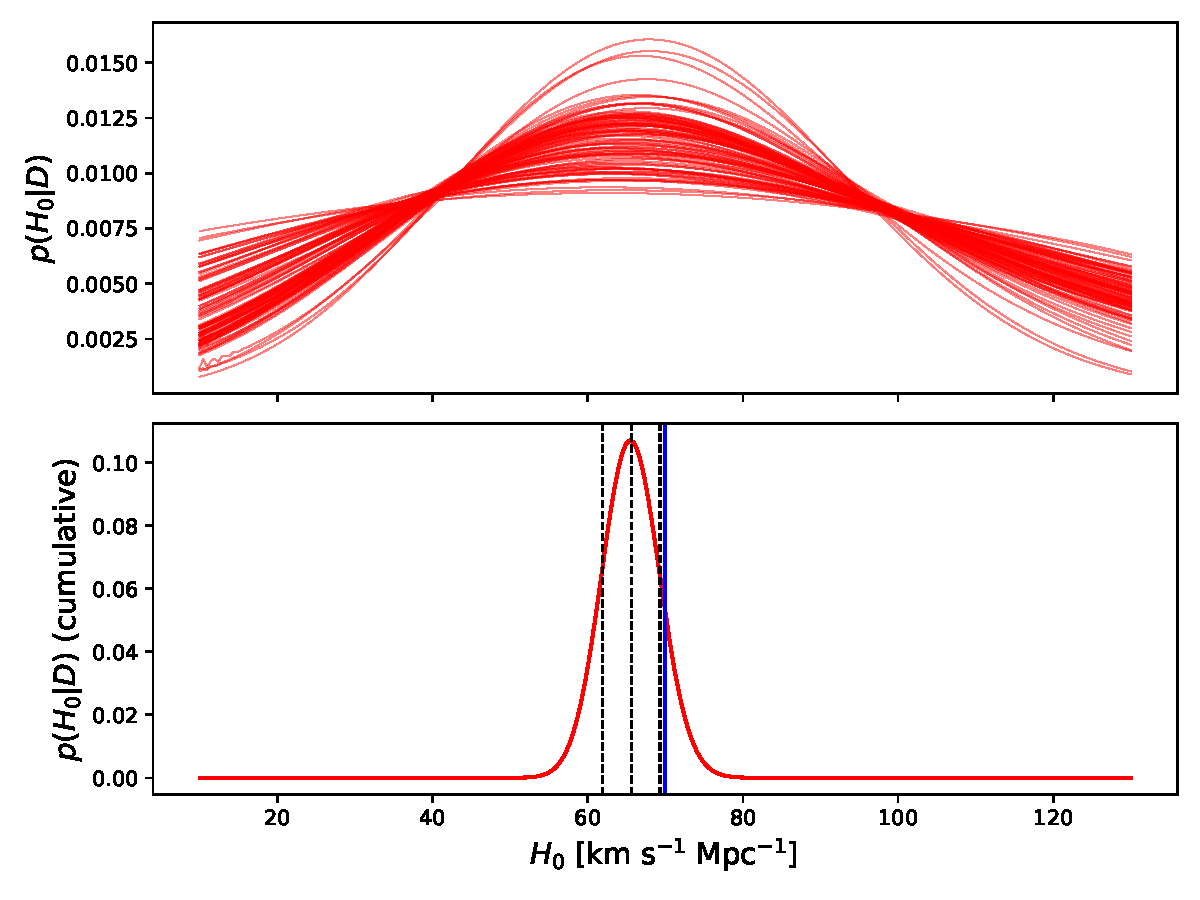
\includegraphics[width=1.5\columnwidth]{figures/posterior.pdf}
    \caption{Upper: Posteriors produced from individual events. The bias of posteriors with poorer localization is noticable, and is probably contributing to the underestimate of $H_0$ that we note. Lower: The posterior $p(H_0 | d_{GW}, d_C)$ produced after $100$ samples. The $68\%$ Confidence interval is shown by the dashed lines. The true injected value is shown in blue.}
    \label{fig:posterior}
\end{figure*}

\begin{figure}
    \centering
    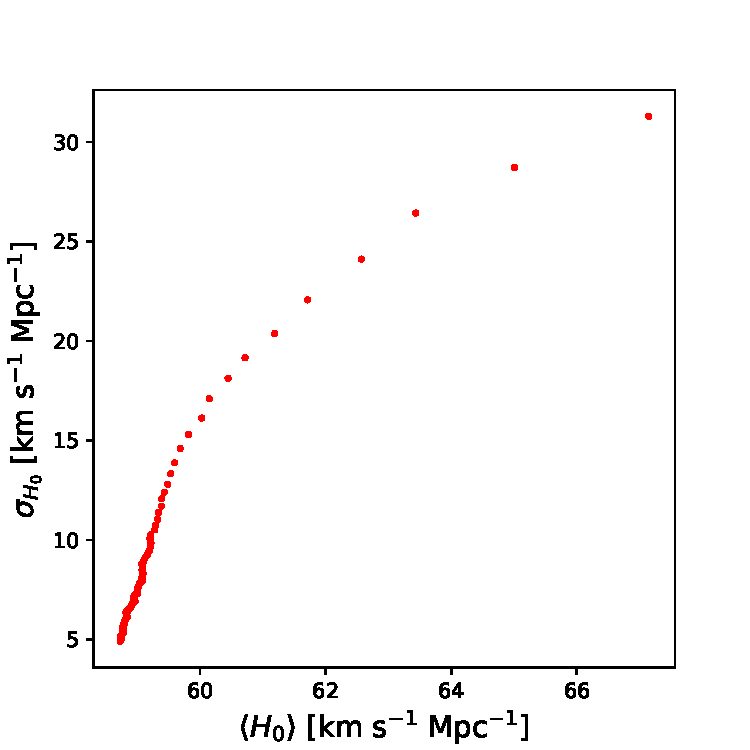
\includegraphics[width=0.95\columnwidth]{figures/correlation.pdf}
    \caption{The means and standard deviations of the estimates on $H_0$ for individual events. Note the clear correlation between these quantities.}
    \label{fig:correlation}
\end{figure}

The resulting posterior $p(H_0 | d_{GW}, d_C)$ produced after $100$ observations is shown in Figure \ref{fig:posterior} along with the posterior obtained from each observation considered in isolation.
In Figure \ref{fig:std} we show the standard deviation of the posterior $p(H_0 | d_{GW}, d_C)$ as a function of number of localized events.
%Some interesting correlations are noticable with events with wider spreads on the posterior tending to center around smaller values of $H_0$.
In Figure \ref{fig:mean_diff} we show the deviation of the posterior expectation on $H_0$ from the known value as a function of number of well localized events.
We can see that our posterior produces an underestimate of $H_0$.
This suggests that there are as yet unidentified systematic effects that need to be taken into account.
Figure \ref{fig:correlation} shows a correlation between the means and standard deviations of the posterior distributions for single events.
This correlation would clearly bias our estimate of $H_0$ towards lower values, since these have smaller standard deviations and thus higher constraining power.
The origin of this correlation is therefore likely to be the unidentified systematic effect.
